\documentclass[english,floatsintext,man]{apa6}

\usepackage{amssymb,amsmath}
\usepackage{ifxetex,ifluatex}
\usepackage{fixltx2e} % provides \textsubscript
\ifnum 0\ifxetex 1\fi\ifluatex 1\fi=0 % if pdftex
  \usepackage[T1]{fontenc}
  \usepackage[utf8]{inputenc}
\else % if luatex or xelatex
  \ifxetex
    \usepackage{mathspec}
    \usepackage{xltxtra,xunicode}
  \else
    \usepackage{fontspec}
  \fi
  \defaultfontfeatures{Mapping=tex-text,Scale=MatchLowercase}
  \newcommand{\euro}{€}
\fi
% use upquote if available, for straight quotes in verbatim environments
\IfFileExists{upquote.sty}{\usepackage{upquote}}{}
% use microtype if available
\IfFileExists{microtype.sty}{\usepackage{microtype}}{}

% Table formatting
\usepackage{longtable, booktabs}
\usepackage{lscape}
% \usepackage[counterclockwise]{rotating}   % Landscape page setup for large tables
\usepackage{multirow}		% Table styling
\usepackage{tabularx}		% Control Column width
\usepackage[flushleft]{threeparttable}	% Allows for three part tables with a specified notes section
\usepackage{threeparttablex}            % Lets threeparttable work with longtable

% Create new environments so endfloat can handle them
% \newenvironment{ltable}
%   {\begin{landscape}\begin{center}\begin{threeparttable}}
%   {\end{threeparttable}\end{center}\end{landscape}}

\newenvironment{lltable}
  {\begin{landscape}\begin{center}\begin{ThreePartTable}}
  {\end{ThreePartTable}\end{center}\end{landscape}}




% The following enables adjusting longtable caption width to table width
% Solution found at http://golatex.de/longtable-mit-caption-so-breit-wie-die-tabelle-t15767.html
\makeatletter
\newcommand\LastLTentrywidth{1em}
\newlength\longtablewidth
\setlength{\longtablewidth}{1in}
\newcommand\getlongtablewidth{%
 \begingroup
  \ifcsname LT@\roman{LT@tables}\endcsname
  \global\longtablewidth=0pt
  \renewcommand\LT@entry[2]{\global\advance\longtablewidth by ##2\relax\gdef\LastLTentrywidth{##2}}%
  \@nameuse{LT@\roman{LT@tables}}%
  \fi
\endgroup}


  \usepackage{graphicx}
  \makeatletter
  \def\maxwidth{\ifdim\Gin@nat@width>\linewidth\linewidth\else\Gin@nat@width\fi}
  \def\maxheight{\ifdim\Gin@nat@height>\textheight\textheight\else\Gin@nat@height\fi}
  \makeatother
  % Scale images if necessary, so that they will not overflow the page
  % margins by default, and it is still possible to overwrite the defaults
  % using explicit options in \includegraphics[width, height, ...]{}
  \setkeys{Gin}{width=\maxwidth,height=\maxheight,keepaspectratio}
\ifxetex
  \usepackage[setpagesize=false, % page size defined by xetex
              unicode=false, % unicode breaks when used with xetex
              xetex]{hyperref}
\else
  \usepackage[unicode=true]{hyperref}
\fi
\hypersetup{breaklinks=true,
            pdfauthor={},
            pdftitle={Bayesian sampling in the interpretation of quantifiers? Evidence from Markov chain Monte Carlo with People},
            colorlinks=true,
            citecolor=blue,
            urlcolor=blue,
            linkcolor=black,
            pdfborder={0 0 0}}
\urlstyle{same}  % don't use monospace font for urls

\setlength{\parindent}{0pt}
%\setlength{\parskip}{0pt plus 0pt minus 0pt}

\setlength{\emergencystretch}{3em}  % prevent overfull lines

\ifxetex
  \usepackage{polyglossia}
  \setmainlanguage{}
\else
  \usepackage[english]{babel}
\fi

% Manuscript styling
\captionsetup{font=singlespacing,justification=justified}
\usepackage{csquotes}
\usepackage{upgreek}



\usepackage{tikz} % Variable definition to generate author note

% fix for \tightlist problem in pandoc 1.14
\providecommand{\tightlist}{%
  \setlength{\itemsep}{0pt}\setlength{\parskip}{0pt}}

% Essential manuscript parts
  \title{Bayesian sampling in the interpretation of quantifiers? Evidence from
Markov chain Monte Carlo with People}

  \shorttitle{Markov chain Monte Carlo with People}


  \author{Fabian Dablander\textsuperscript{1}}

  \def\affdep{{""}}%
  \def\affcity{{""}}%

  \affiliation{
    \vspace{0.5cm}
          \textsuperscript{1} University of Tübingen  }

  \authornote{
    \newcounter{author}
    This research was conducted during an internship supervised by Dr.~phil
    Michael Franke at the University of Tübingen. Most of the ideas
    presented here are his. I want to thank him for his creative input and
    patience.

                      Correspondence concerning this article should be addressed to Fabian Dablander. E-mail: \href{mailto:dablander.fabian@gmail.com}{\nolinkurl{dablander.fabian@gmail.com}}
                }


  \abstract{How do people use quantifiers such as \emph{some} and \emph{many}?
Within the growing discipline of probabilistic pragmatics, we take first
steps in answering this question by comparing three Bayesian models that
estimate participants' subjective probability distribution of ten
different quantifiers. We use an experimental design in which
participants' responses are viewed as states in a Markov chain Monte
Carlo algorithm---``Markov chain Monte Carlo with People'' (Sanborn \&
Griffiths, 2007). Fourty-five participants were presented with fifty
forced-choice trials for four different, randomly chosen quantifiers in
which two images were presented which displayed different numbers of red
dots. Participants had to indicate which image was a better description
for the specific quantifier in use. Three models of the data generating
process were developed. Interestingly, the model which closely mirrors
the experimental design and assumes participants are Bayesian samplers
had higher prediction error than a model which assumes participants
soft-max prefer the number which is closer to the mode of the subjective
probability distribution. Limitations of our preliminary finding as well
as implications for further research are discussed.}
  \keywords{Bayesian modeling, experimental pragmatics, quantifier interpretation,
Markov chain Monte Carlo with People \\

    \indent Word count: 2554
  }




  \usepackage{setspace}
  \usepackage{rotating}
  \usepackage{algorithm}
  \usepackage{algpseudocode}

\begin{document}

\maketitle

\setcounter{secnumdepth}{0}



How do people interpret quantifiers? Say I arrive hungry at a party
where I gleefully discover twelve cookies on the kitchen table. The
host, recognising my desire, says that I can have \emph{some}. Can I eat
two? Sure. What about ten? Probably not.

Why does two seem more likely than ten? Following the data-oriented
approach of probabilistic pragmatics (Franke \& Jäger, 2016), we tackle
this question by estimating the subjective probability distribution over
possible values (in the above example: cookies) for different
quantifiers. To arrive at this distribution, we utilize an experimental
design which uses participants' answers as states in a Markov chain
Monte Carlo (MCMC) algorithm---\enquote{Markov chain Monte Carlo with
People} (Sanborn \& Griffiths, 2007). Additionally, we develope three
Bayesian models of the data generating process, and directly test the
hypothesis of a \enquote{Bayesian brain} (Sanborn \& Chater, 2016) in
quantifier use. Let's unpack the underlying ideas in turn.

\subsubsection{Bayesian inference}\label{bayesian-inference}

Bayesian approaches are becoming increasingly popular as (a) an
alternative to classical statistical data analysis (Wagenmakers et al.,
2015), (b) a tool to estimate (hierarchical) cognitive models (Lee,
2011), and (c) a theory about how the brain works (Sanborn \& Chater,
2016). The latter idea is known as the \enquote{Bayesian brain}, a theme
that offers to unify different aspects of cognition (Chater, Oaksford,
Hahn, \& Heit, 2010); the brain is viewed as a Bayesian inference
machine which approximates complex probability distributions.

The most common objection to this idea is the observation that human
cognition seems far from \emph{optimal} or \emph{rational} (Marcus,
2009; Marcus \& Davis, 2013); instead, it seems more plausible to assume
that our actions are guided by evolved satisficing strategies that lead
to common reasoning errors such as the conjunction fallacy (e.g.,
Tversky \& Kahneman, 1983). In a recent paper, however, Sanborn \&
Chater (2016) explain these satisficing strategies and the resulting
reasoning errors by viewing the brain not as an ideal Bayesian reasoner,
but as Bayesian sampler. Only asymptotically do we follow the rules of
probability exactly and act according to rational choice; with finite
time and, thus, finite samples, reasoning errors result.

In this paper, we seek to directly test the notion that participants are
Bayesian samplers in the domain of quantifier interpretation. We utilize
an experimental design---\enquote{Markov chain Monte Carlo with People}
(Sanborn \& Griffiths, 2007)---which is inspired by computational
challenges of Bayesian inference, and which allows us to sample from the
subjective probability distribution of quantifiers.

Bayesian inference starts with a prior belief \(p(\theta)\) over some
parameter vector \(\theta\). The likelihood function
\(\mathcal{L}(\theta|\textbf{y})\) specifies how the parameter vector
relates to the observed data \(\textbf{y}\). Combining the two using
Bayes' rule two yields the posterior distribution over the parameter
vector, \(p(\theta|\textbf{y})\):

\[
p(\theta|\textbf{y}) = \frac{p(\theta)\mathcal{L}(\theta|\textbf{y})}{\int p(\theta)\mathcal{L}(\theta|\textbf{y})\mathrm{d}\theta}
\]

In most cases, the denominator is a high dimensional integral which
cannot be calculated analytically. To this end, sampling-based methods
such as Markov chain Monte Carlo techniques are used which avoid
computing the integral altogether (for an introduction, see e.g.,
Ravenzwaaij, Cassey, \& Brown, 2016). Concretely, one sets up a Markov
chain which has as its stationary distribution the normalized posterior
distribution \(p(\theta|\textbf{y})\). Various algorithms have been
proposed, but the canonical one is the Metropolis-Hastings (MH) method
(Hastings, 1970; Metropolis, Rosenbluth, Rosenbluth, Teller, \& Teller,
1953).

\subsubsection{Metropolis-Hastings}\label{metropolis-hastings}

The key insight here is that we do not need to have access to the
posterior distribution but need only be able to compute its density,
\(\pi(x)\), for values of \(x\). The MH algorithm works as follows (see
also the pseudocode below). Start at random initial state \(x\). In each
step, generate a new sample \(x^{\star}\) based on the current value
using a proposal function. Choose \(x^{\star}\) over \(x\) using a
specified acceptance function. Required some mathematical conditions
(see e.g., Jackman, 2009, p. 201), this constitutes a Markov chain of
first order which has \(p(\theta|\textbf{y})\) as its stationary
distribution. Once the stationary distribution is reached, the generated
samples are equivalent to samples from \(p(\theta|\textbf{y})\). The
samples before that time in point are discarded as \enquote{burn-in}.

If we further assume that the probability of proposing a new state
\(x^{\star}\) based on the current state \(x\) is the same as the
probability of proposing \(x\) based on \(x^{\star}\), i.e., the
proposal distribution is symmetric, we can use the Barker acceptance
function (Barker, 1965)

\[
A(x; x^{\star}) = \frac{\pi(x^{\star})}{\pi(x^{\star}) + \pi(x)}
\]

where \(\pi(x)\) indicates the density of the value \(x\) under the
posterior distribution.

\begin{spacing}{0.8}
\begin{algorithm}[ht]
    \caption{Barker Random-Walk Metropolis-Hasting}
    
    \begin{algorithmic}
    
        \Procedure{Metropolis}{$\sigma, N$}
          \State $\mbox{samples[1]} \gets \mbox{RandomState()}$
          \State $\mbox{samples[2:N]} \gets 0$
          \For{$i = 2$ to $N$}
              \State $x \gets \mbox{samples[i - 1]}$
              \State $x^{\star} \gets x + \mbox{Normal(}\mu = 0, \sigma = \sigma\mbox{)}$
              \State $A \gets \frac{\pi(x^{\star})}{\pi(x^{\star}) + \pi(x)}$
              
              \If{$A \geq \mbox{Uniform(0, 1)}$}
                  \State $\mbox{samples[i]} \gets x^{\star}$
              \Else
                  \State $\mbox{samples[i]} \gets x$
              \EndIf
              
          \EndFor
          
      \State \textbf{return} samples
      
      \EndProcedure
    \end{algorithmic}
\end{algorithm}
\end{spacing}

In our experimental design we use participants' responses as states in a
Markov chain, with the stationary distribution being the subjective
probability distribution over values provided a specific quantifier. We
then estimate three models of the data generating process. One of them,
referred to as the Barker model, describes the experimental design. If
participants are Bayesian samplers, this model should describe the data
best.

The document was written in a reproducible manner using Rmarkdown and
the papaja R package (Aust \& Barth, 2016). All materials, including
data, code for the experiment and data analysis, and manuscript, can be
found at
\mbox{\href{https://github.com/fdabl/MCMCP}{https://github.com/fdabl/MCMCP}}.

\section{Methods}\label{methods}

We report how we determined our sample size, all data exclusions, all
manipulations, and all measures in the study. In a pilot study, five
participants were recruited in order to test the technical setup of the
experiment. Those participants are not included in the final analysis.

\subsection{Participants}\label{participants}

Fifty participants were recruited from Amazon Mechanical Turk
(Buhrmester, Kwang, \& Gosling, 2011). After inspection of the data,
five participants were
removed\footnote{See appendix for the rationale and the excluded participants' data patterns.},
leaving a total of fourty-five participants. On average, the experiment
took 9.38 minutes to complete. The experiment seemed to be engaging and
not too difficult (Mean engagement = 7.35, Mean difficulty = 3.73;
scale: 1-10). Fourty-two Participants were self-reported native English
speakers, three were of different mother tongue (French, Romanian,
Russian).

\subsection{Material}\label{material}

Images of random dot patterns were used. Each image showed 432 dots, of
which any amount could be coloured red. The other dots were coloured
black. For each possible pattern (0 - 432 red dots), ten images were
generated. On each trial, images were randomly chosen out of the
generated pool of images.

\subsection{Procedure}\label{procedure}

After reading the instruction, each participant went through four blocks
of 50 trials each. Each block consisted of a quantifier randomly chosen
out of \emph{Half}, \emph{About half}, \emph{Less than half},
\emph{Few}, \emph{Very few}, \emph{Many}, \emph{Most}, \emph{The
majority}, \emph{Some}, \emph{Almost all}. No participant saw a
quantifier twice, and \emph{About half} was never followed by
\emph{Half} and \emph{Very few} never by \emph{Few} (and vice versa). On
each trial, the participant had to choose which of the two images fitted
the description best (see Figure 1 for an example trial). On the
following trial, new images were generated.

\begin{figure}[htbp]
\centering
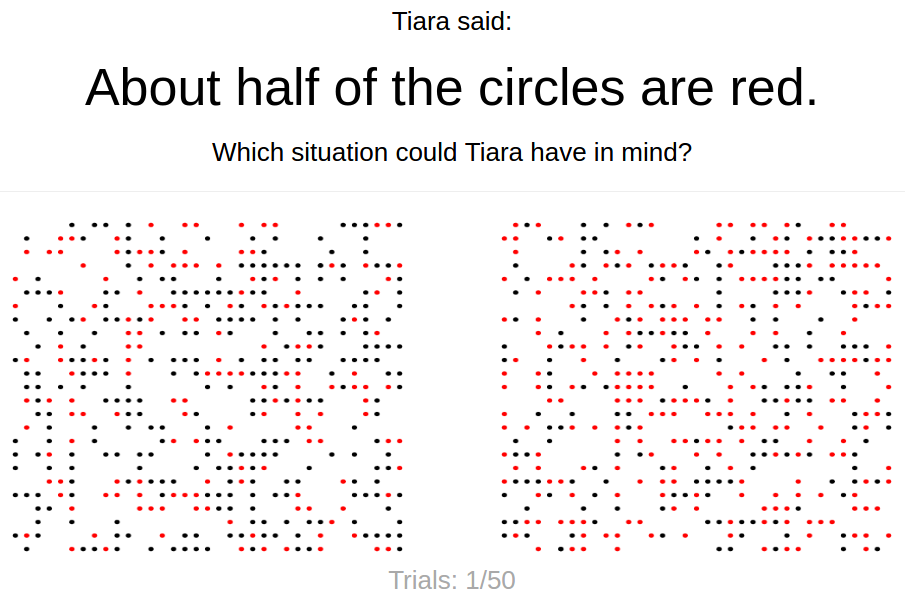
\includegraphics{img/trial-image}
\caption{Example Trial. Participants had to choose between the left or
right image. Names in the description were chosen randomly out of a pool
of fifty names.}
\end{figure}

Analogously to the steps of a MH algorithm, the number of red dots in
the images on the first trial of each block were generated randomly. On
subsequent trials, samples based on the current number of red dots were
proposed. Note that the support of the distribution we want to elicit is
bounded by the interval \([0, 432]\). Therefore, to ensure a symmetric
proposal function, our MH algorithm proceeded as follows. Given the
chosen number of red dots \(x\), uniformly generate points for the
second image within the interval \([x - \delta, x + \delta]\) with
probability \(1 - \epsilon\). With probability \(\epsilon\), points were
generated uniformly outside the interval. Again, symmetry is crucial to
enable the use of the Barker acceptance function. We set \(\delta = 20\)
and \(\epsilon = .4\).

As an example, assume the participant chose the image with 420 red dots.
Out of a hundred cases, in sixty cases the newly selected image will
have points from the set \(\{400, \ldots, 432, 0, \ldots, 8\}\). In
fourty cases, it will have points selected from the set
\(\{8, \ldots, 400\}\).

\begin{figure}[htbp]
\centering
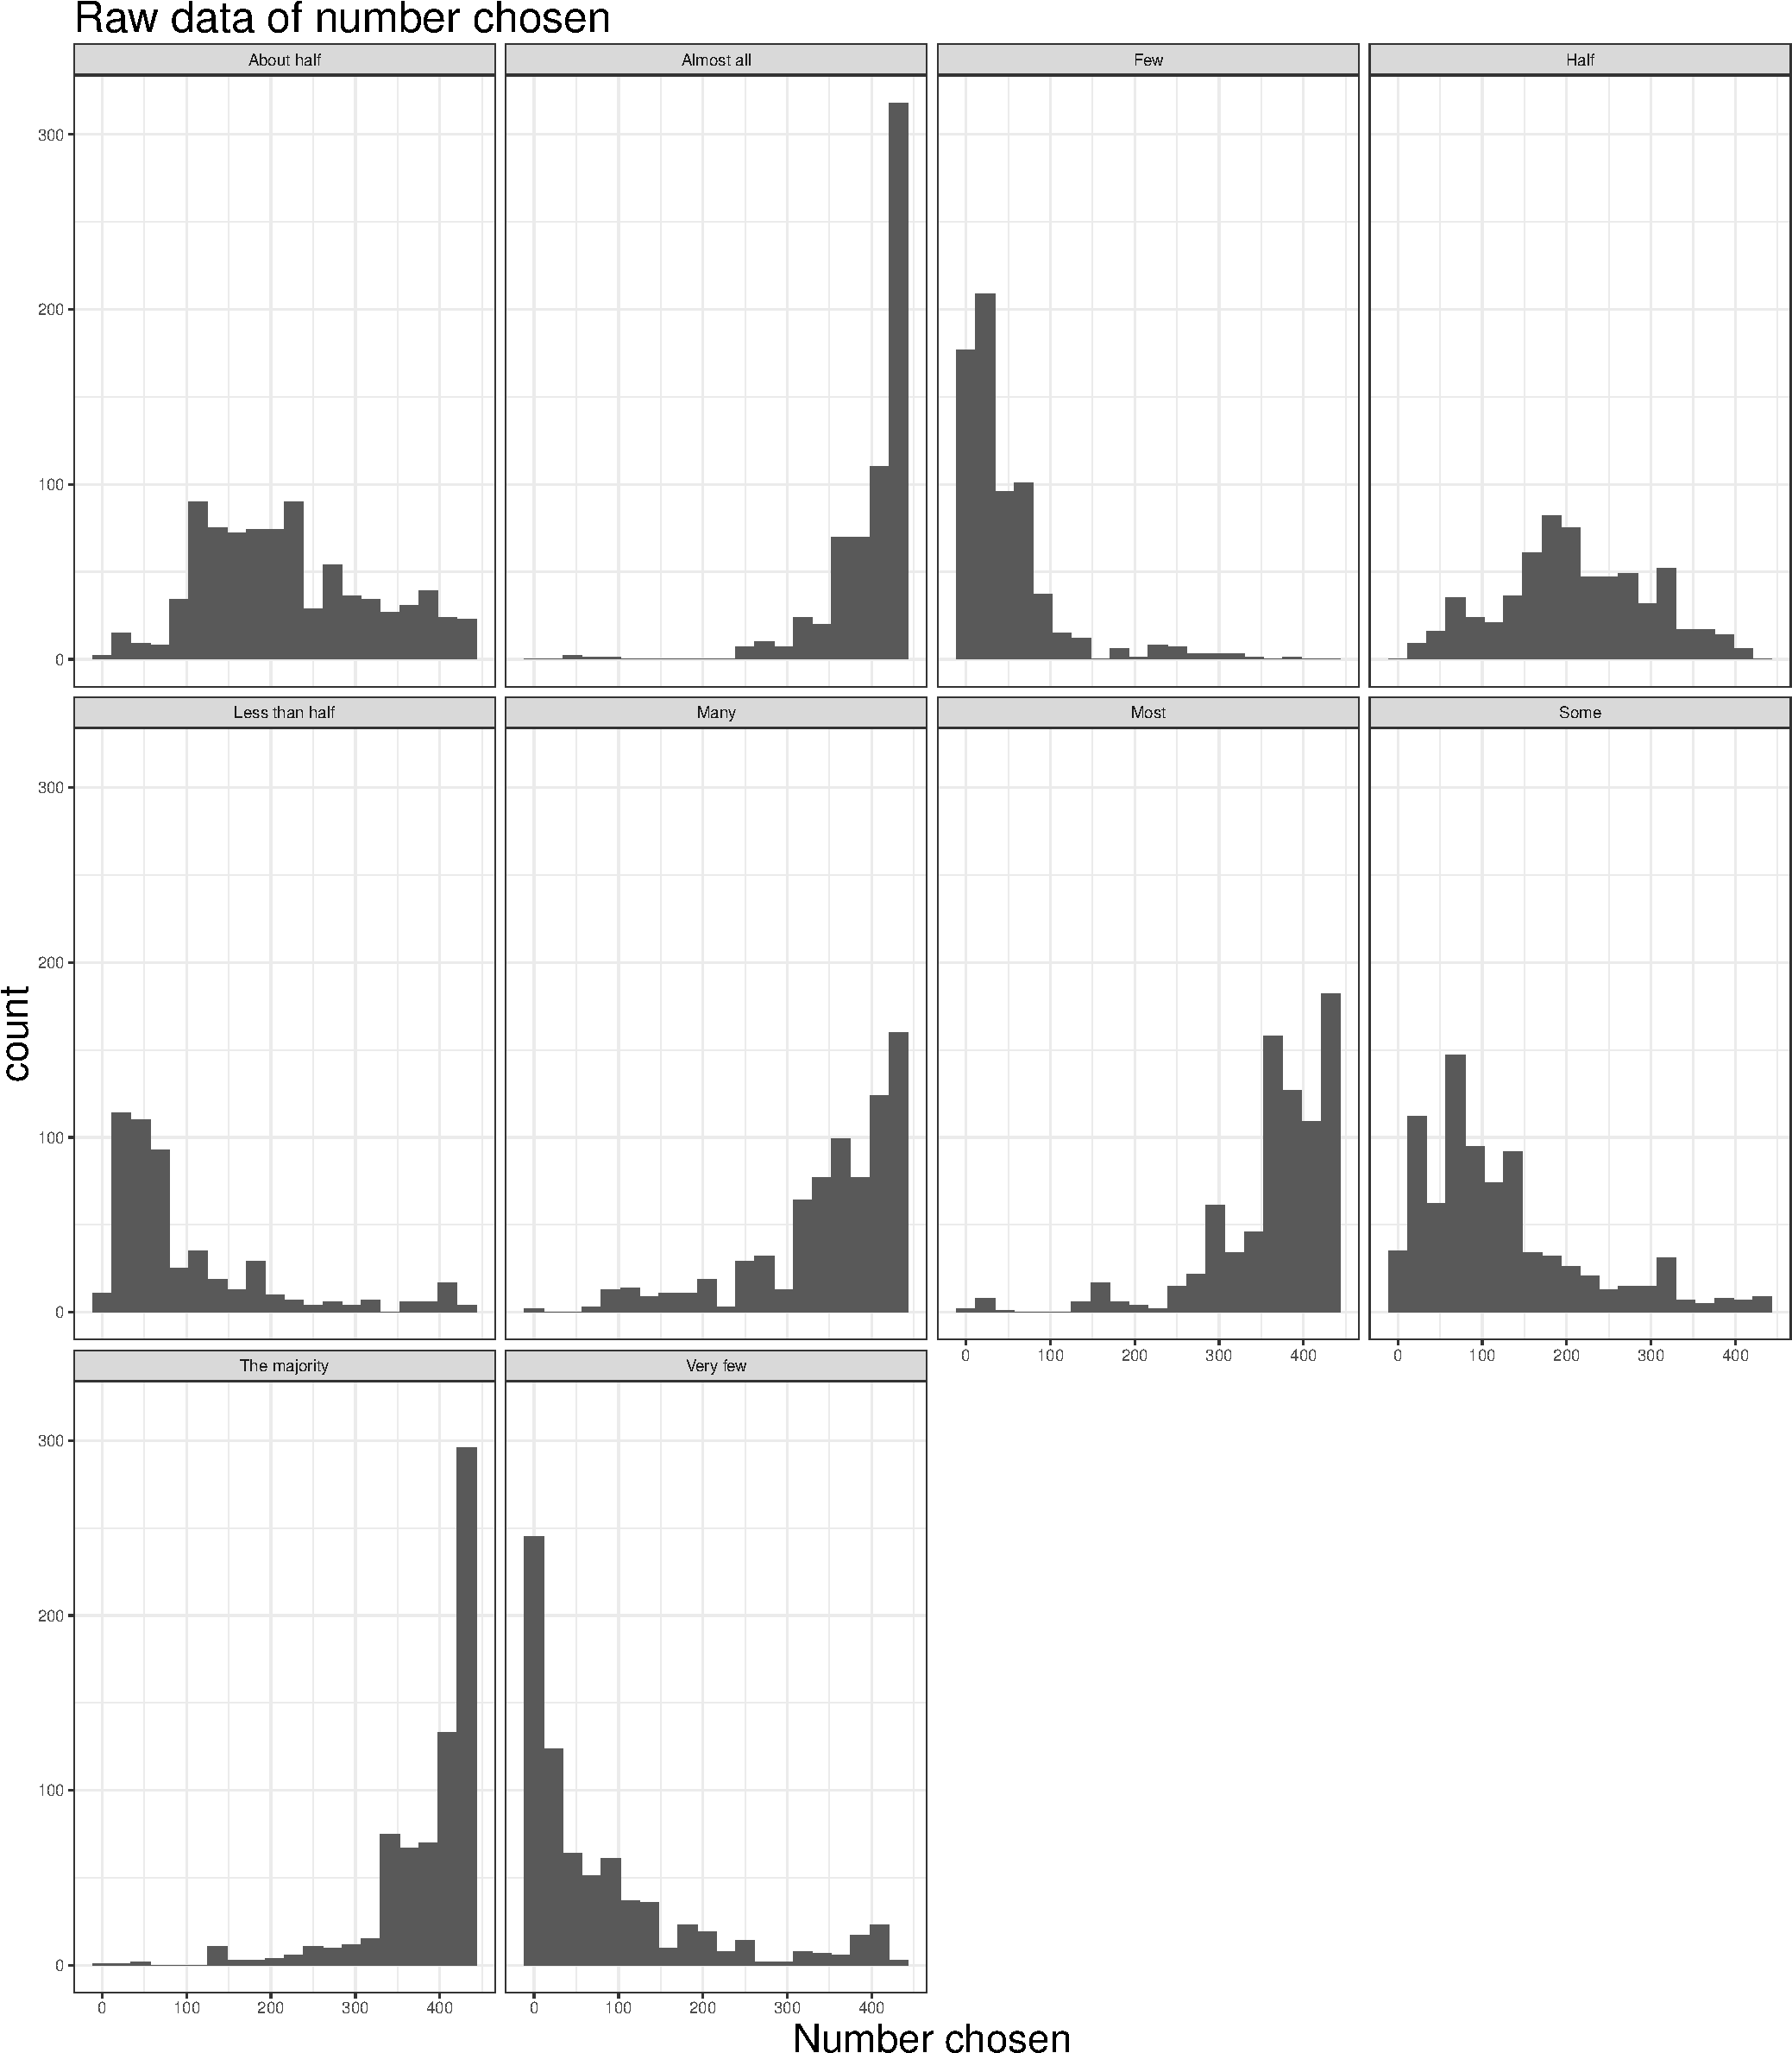
\includegraphics{manuscript_files/figure-latex/unnamed-chunk-5-1.pdf}
\caption{\label{fig:unnamed-chunk-5}Histograms of the raw data (number
chosen) for all quantifiers pooled over participants.}
\end{figure}

\section{Data analysis}\label{data-analysis}

All analyses were completed using the open-source statistical
programming language R (R Core Team, 2016). We removed five participants
whose response pattern was highly unusual (see appendix). The data we
want to explain is the choice the participants make in each trial: do
they pick the image with the higher number of red dots? Figure 2 shows a
visualization of pooled participants' data for all quantifiers. See
Figure 3 for a visualization of participant-wise choice data for the
quantifier \emph{Some}. The full dataset can be interactively explored
at
\mbox{\href{https://fdabl.shinyapps.io/MCMCP/}{https://fdabl.shinyapps.io/MCMCP/}}.

\begin{figure}[htbp]
\centering
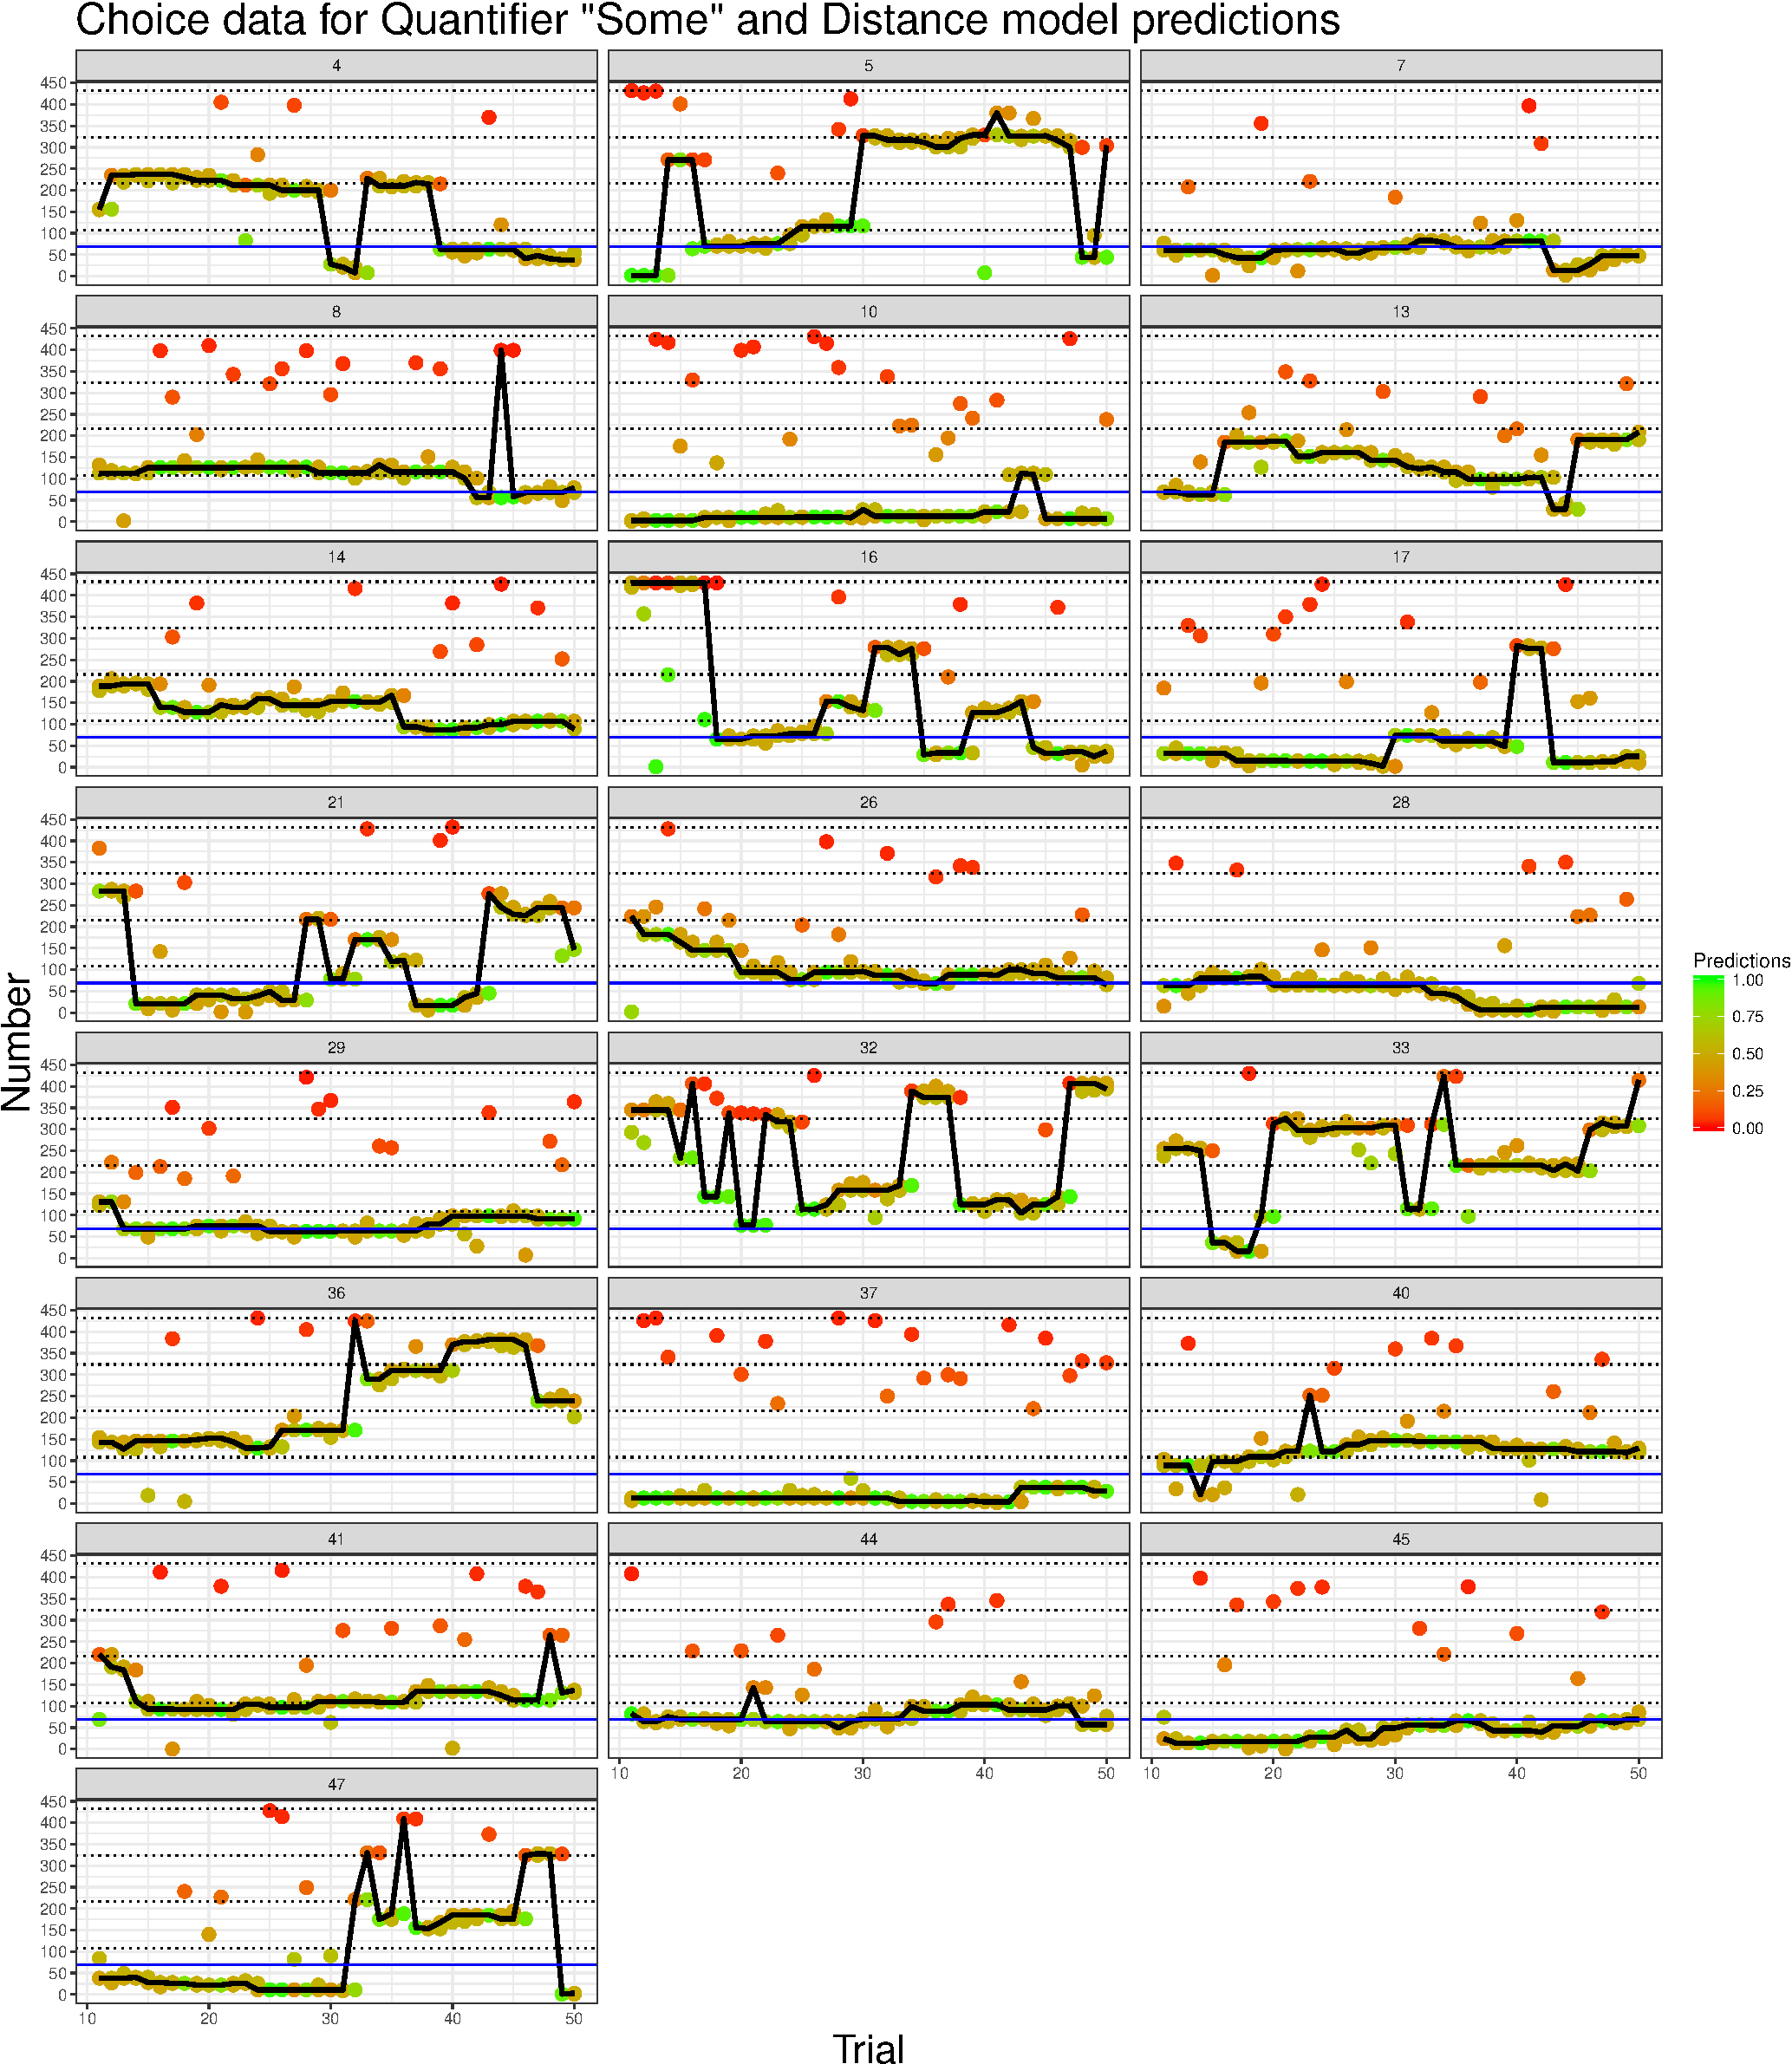
\includegraphics{manuscript_files/figure-latex/unnamed-chunk-6-1.pdf}
\caption{\label{fig:unnamed-chunk-6}Shows the raw data of all participants
who completed a block with the quantifier \emph{Some}. Colour indicates
the predictions of the Distance model for each respective data point.
Blue line indicates the mode of the subjective distribution. Note that
the first ten trials were discarded as burn-in.}
\end{figure}

\subsection{Model specification}\label{model-specification}

\begin{figure}[htbp]
\centering
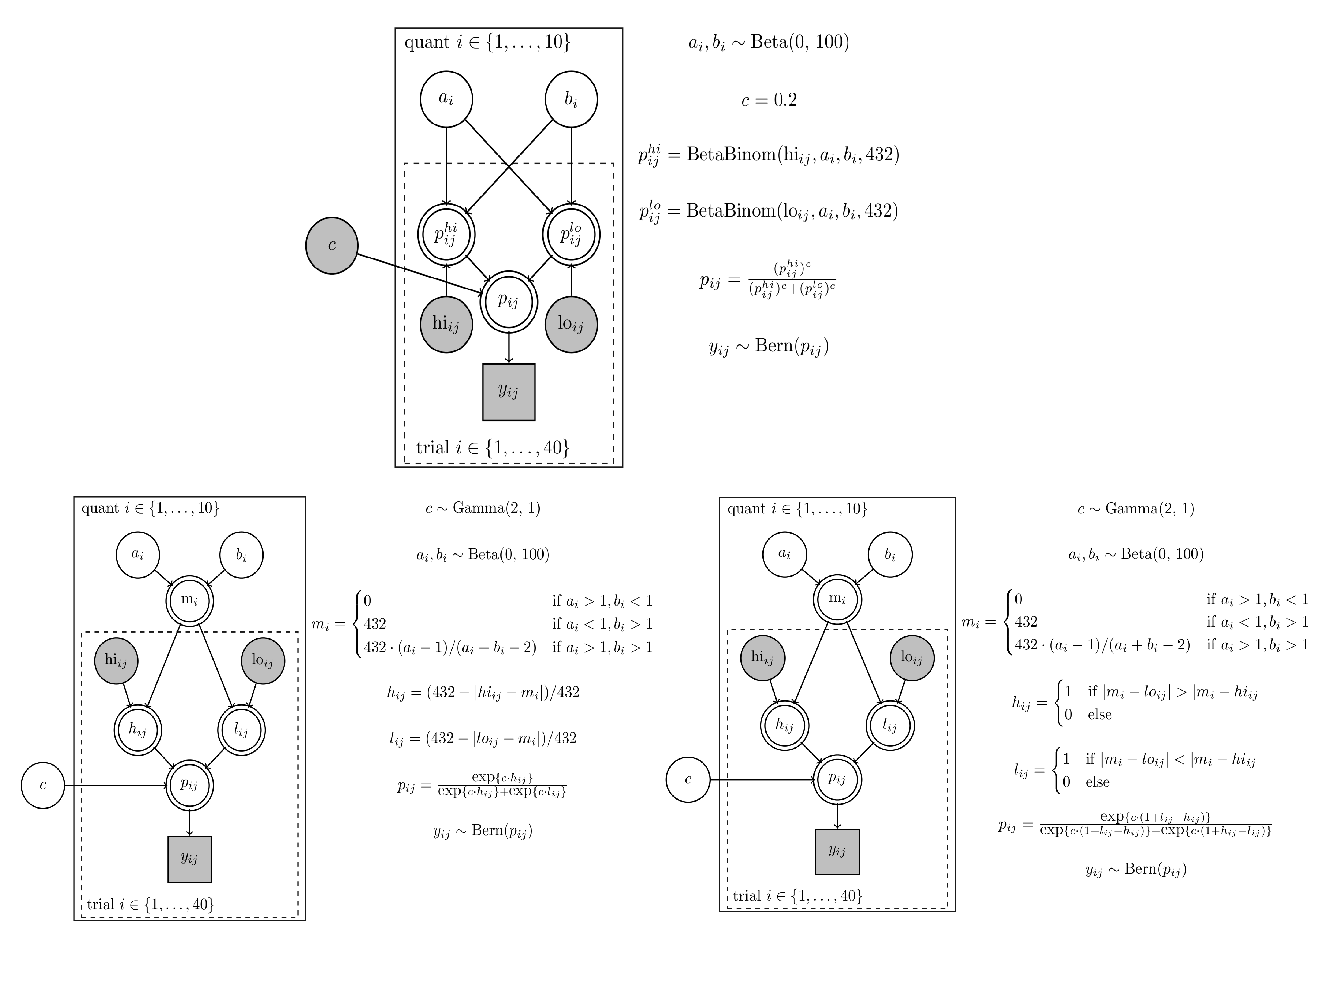
\includegraphics{model_graphs/models_combined.png}
\caption{Graphical model specification for the Barker model (top), the
Distance model (left), and the Closer model (right). Transparent nodes
indicate parameters, shaded ones indicate observed values. Circles
indicate continuous, rectangles categorical values. Nodes with double
lines indicate deterministic nodes.}
\end{figure}

We developed three models of the data generating process. Common to all
is the parameterization of the distribution over number of red dots for
each quantifier as a beta-binomial distribution, and the Bernoulli
likelihood function.

Two of the models, thereafter \emph{Closer model} and \emph{Distance
model}, assume the participant is soft-max preferring the image in which
the number of red dots is closer to the mode of the subjective
distribution for that quantifier. The Distance model uses information
about the distance of the choices to the mode, while the Closer model
uses a categorical measure of distance (closer or not closer). The
models are similar to the one discussed by Franke et al. (2016) for the
\emph{bin comparison} task.

The third model, which we call the \emph{Barker model}, does not use the
mode but instead compares the likelihood of the respective number of red
dots---just like the Barker acceptance function in the MCMC algorithm.
See Figure 4 for the graphical model specifications using the notation
of Lee \& Wagenmakers (2014).

\subsection{Model inference}\label{model-inference}

We used JAGS (Plummer, 2003) to estimate the model parameters. 100.000
samples were obtained from two chains with a thinning rate of 2 after
burn-in of 5000 that ensured convergence according to \(\hat R\) (Gelman
\& Rubin, 1992) for the Distance and Closer model. Even after increasing
the samples to 200.000, the Barker model did not converge. This was
because the parameters were underspecified; different values for \(a\),
\(b\), and \(c\) resulted in the same likelihood. Therefore, we set the
parameter \(c = 1\) which resulted in
convergence\footnote{Changing the parameter to c = .2 or c = .5 did not alter the main conclusion drawn. However, the model fitted best with $c = .2$; we report conclusions based on this fit.}.

\section{Results and Discussion}\label{results-and-discussion}

We compared the models using the likelihood as well as the Deviance
Information Criterion (DIC; Spiegelhalter, Best, Carlin, \& Van Der
Linde, 2002), the latter being an estimate for out of sample prediction
error. The Distance model had lower prediction error than the Closer
model (see Table 1). This is not surprising, because the Distance model
uses information about the numerical distance of the choices to the
mode, while the Closer model only cares about which choice is closer.
Interestingly, the Distance model fares better than the Barker model.
Note again that the Barker model closely mirrors the experimental
design.

\begin{table}[tbp]
\begin{center}
\begin{threeparttable}
\caption{Results of model comparison.}
\begin{tabular}{llll}
\toprule
 & \multicolumn{1}{c}{Distance} & \multicolumn{1}{c}{Barker} & \multicolumn{1}{c}{Closer}\\
\midrule
DIC & 7848.373 & 8194.429 & 8654.730\\
Likelihood & 4963.402 & 4690.150 & 4669.204\\
\bottomrule
\end{tabular}
\end{threeparttable}
\end{center}
\end{table}

The underspecification of parameters with \(c\) as a free parameter in
the Barker model required us to specify contraints. We did this by
fixing \(c\); \(c\) influences how strongly participants prefer higher
values. For \(c\) approaching zero, participants have no preference,
i.e.~there choice whether to prefer the image with the higher number of
red dots or the image with the lower number of red dots was random; for
\(c\) greater than one, participants prefer higher values. The
prediction error as measured by the DIC decreased with a decreasing
\(c\), indicating that the Barker model did not capture relevant
regularities in the data.

Although we want to avoid drawing strong conclusions from these
preliminary results, it seems that, in contrast to what the
\enquote{Bayesian brain} hypothesis postulates, participants do not
engage in sampling-based algorithmic behaviour in the domain of
quantifier interpretation. Instead, it seems that participants infer
likely values given the quantifier based on the distance to the mode of
the subjective distribution over all values under that quantifier.

There are a number of limitations that need to be addressed. With
respect to the experimental design, it is unclear how many trials are
needed for the Markov chain to converge, and for the resulting samples
to be draws from the subjective probability distribution. In our
analysis, we excluded the first ten trials as burn-in, only working with
the resulting fourty. Other choices might be equally, or more
reasonable. This point is exaggerated by the observation that
participant's choices are---by design---not independent; there is serial
autocorrelation which violates our assumption of an independent
Bernoulli likelihood. Along the same lines, it is unclear whether our
parameter settings \(\delta = 20\) and \(\epsilon = .4\) for the
proposal function which generated new images are adequate, i.e.~whether
this results in a good exploration of the state space.

However, these issues are analogous to the issues in Markov chain Monte
Carlo based inference more broadly, an area where remedies have already
been developed; future research should utilize approaches from this
domain. For example, to assess convergence, one could repeatedly present
the participants with blocks of the same quantifier, i.e.~run more than
one Markov chain, and compute statistics such as \(\hat R\) (Gelman \&
Rubin, 1992).

In this paper, we assumed that participants share the same probability
distribution over the number of red dots for each quantifier; this
simplifying assumption need not be reasonable. Future research should
utilize a hierarchical approach similar to Franke et al. (2016),
estimating individual-level probability distribution as variations of a
shared population-level belief.

Despite the limitations, we believe that this paper constitutes a novel
contribution by extending the use of Markov chain Monte Carlo with
People type experiments to the domain of language interpretation.
Moreover, it casts initial doubt on the idea of the brain as a Bayesian
sampler in quantifier interpretation. Avenues for future research
abound.

\section{References}\label{references}

\setlength{\parindent}{-0.5in} \setlength{\leftskip}{0.5in}

\hypertarget{refs}{}
\hypertarget{ref-R-papaja}{}
Aust, F., \& Barth, M. (2016). \emph{papaja: Create APA manuscripts with
RMarkdown}. Retrieved from \url{https://github.com/crsh/papaja}

\hypertarget{ref-barker1965monte}{}
Barker, A. (1965). Monte Carlo calculations of the radial distribution
functions for a proton? electron plasma. \emph{Australian Journal of
Physics}, \emph{18}(2), 119--134.

\hypertarget{ref-buhrmester2011amazon}{}
Buhrmester, M., Kwang, T., \& Gosling, S. D. (2011). Amazon's Mechanical
Turk a new source of inexpensive, yet high-quality, data?
\emph{Perspectives on Psychological Science}, \emph{6}(1), 3--5.
doi:\href{https://doi.org/10.1177/1745691610393980}{10.1177/1745691610393980}

\hypertarget{ref-chater2010bayesian}{}
Chater, N., Oaksford, M., Hahn, U., \& Heit, E. (2010). Bayesian models
of cognition. \emph{Wiley Interdisciplinary Reviews: Cognitive Science},
\emph{1}(6), 811--823.
doi:\href{https://doi.org/10.1002/wcs.79}{10.1002/wcs.79}

\hypertarget{ref-franke2016probabilistic}{}
Franke, M., \& Jäger, G. (2016). Probabilistic pragmatics, or why Bayes'
rule is probably important for pragmatics. \emph{Zeitschrift Für
Sprachwissenschaft}, \emph{35}(1), 3--44.
doi:\href{https://doi.org/10.1515/zfs-2016-0002}{10.1515/zfs-2016-0002}

\hypertarget{ref-franke2016cogsci}{}
Franke, M., Dablander, F., Schöller, A., Bennett, E., Degen, J.,
Henry-Tessler, M., \ldots{} Goodman, N. D. (2016). What does the crowd
believe? A hierarchical approach to estimating subjective beliefs from
empirical data. In Papafragou A., Grodner D., Mirman D., \& T. J. C.
(Eds.), \emph{Proceedings of the 38th Annual Conference of the Cognitive
Science Society} (pp. 2669--2674).

\hypertarget{ref-gelman1992inference}{}
Gelman, A., \& Rubin, D. B. (1992). Inference from iterative simulation
using multiple sequences. \emph{Statistical Science}, 457--472.

\hypertarget{ref-hastings1970monte}{}
Hastings, W. K. (1970). Monte Carlo sampling methods using Markov chains
and their applications. \emph{Biometrika}, \emph{57}(1), 97--109.

\hypertarget{ref-jackman2009bayesian}{}
Jackman, S. (2009). \emph{Bayesian analysis for the social sciences}
(Vol. 846). John Wiley \& Sons.

\hypertarget{ref-lee2011cognitive}{}
Lee, M. D. (2011). How cognitive modeling can benefit from hierarchical
Bayesian models. \emph{Journal of Mathematical Psychology}, \emph{55},
1--7.
doi:\href{https://doi.org/10.1016/j.jmp.2010.08.013}{10.1016/j.jmp.2010.08.013}

\hypertarget{ref-lee2014bayesian}{}
Lee, M. D., \& Wagenmakers, E. (2014). \emph{Bayesian cognitive
modeling: A practical course}. Cambridge University Press.

\hypertarget{ref-marcus2009kluge}{}
Marcus, G. (2009). \emph{Kluge: The haphazard evolution of the human
mind}. Houghton Mifflin Harcourt.

\hypertarget{ref-marcus2013robust}{}
Marcus, G., \& Davis, E. (2013). How robust are probabilistic models of
higher-level cognition? \emph{Psychological Science}, \emph{24}(12),
2351--2360.
doi:\href{https://doi.org/10.1177/0956797613495418}{10.1177/0956797613495418}

\hypertarget{ref-metropolis1953equation}{}
Metropolis, N., Rosenbluth, A. W., Rosenbluth, M. N., Teller, A. H., \&
Teller, E. (1953). Equation of state calculations by fast computing
machines. \emph{The Journal of Chemical Physics}, \emph{21}(6),
1087--1092.

\hypertarget{ref-plummer2003jags}{}
Plummer, M. (2003). JAGS: A program for analysis of Bayesian graphical
models using Gibbs sampling. In \emph{Proceedings of the 3rd
international workshop on distributed statistical computing} (Vol. 124,
p. 125).

\hypertarget{ref-R-base}{}
R Core Team. (2016). \emph{R: A language and environment for statistical
computing}. Vienna, Austria: R Foundation for Statistical Computing.
Retrieved from \url{https://www.R-project.org/}

\hypertarget{ref-ravenzwaaij2016simple}{}
Ravenzwaaij, D., Cassey, P., \& Brown, S. D. (2016). A simple
introduction to Markov Chain Monte--Carlo sampling. \emph{Psychonomic
Bulletin \& Review}, 1--12.
doi:\href{https://doi.org/10.3758/s13423-016-1015-8}{10.3758/s13423-016-1015-8}

\hypertarget{ref-sanborn2016bayesian}{}
Sanborn, A. N., \& Chater, N. (2016). Bayesian brains without
probabilities. \emph{Trends in Cognitive Sciences}, \emph{20}(12),
883--893.
doi:\href{https://doi.org/10.1016/j.tics.2016.10.003}{10.1016/j.tics.2016.10.003}

\hypertarget{ref-sanborn2007markov}{}
Sanborn, A. N., \& Griffiths, T. L. (2007). Markov chain Monte Carlo
with People. In \emph{Advances in neural information processing systems}
(pp. 1265--1272).

\hypertarget{ref-spiegelhalter2002bayesian}{}
Spiegelhalter, D. J., Best, N. G., Carlin, B. P., \& Van Der Linde, A.
(2002). Bayesian measures of model complexity and fit. \emph{Journal of
the Royal Statistical Society: Series B (Statistical Methodology)},
\emph{64}(4), 583--639.

\hypertarget{ref-tversky1983extensional}{}
Tversky, A., \& Kahneman, D. (1983). Extensional versus intuitive
reasoning: The conjunction fallacy in probability judgment.
\emph{Psychological Review}, \emph{90}(4), 293--315.

\hypertarget{ref-wagenmakers2015need}{}
Wagenmakers, E., Verhagen, A., Ly, A., Matzke, D., Steingroever, H.,
Rouder, J., \& Morey, R. (2015). The need for Bayesian hypothesis
testing in psychological science. In Papafragou A., Grodner D., Mirman
D., \& T. J. C. (Eds.), \emph{Psychological science under scrutiny:
Recent challenges and proposed solutions}. John Wiley \& Sons.





  \begin{appendix}
  \section{}
  The figure below shows the raw choice data for the participants that
  have been excluded. An online app where the full dataset can be
  interactively explored is hosted at
  \mbox{\href{https://fdabl.shinyapps.io/MCMCP/}{https://fdabl.shinyapps.io/MCMCP/}}.
  All materials are available at
  \mbox{\href{https://github.com/fdabl/MCMCP}{https://github.com/fdabl/MCMCP}}.
  
  The participant on the top left was excluded due to a bias towards small
  values, while three other participants were excluded due to a bias
  towards large values. The fifth participant who was excluded did not
  seem to understand the experiment, unsystematically alternating between
  images with a higher and lower number of red dots.
  
  \begin{figure}
  \centering
  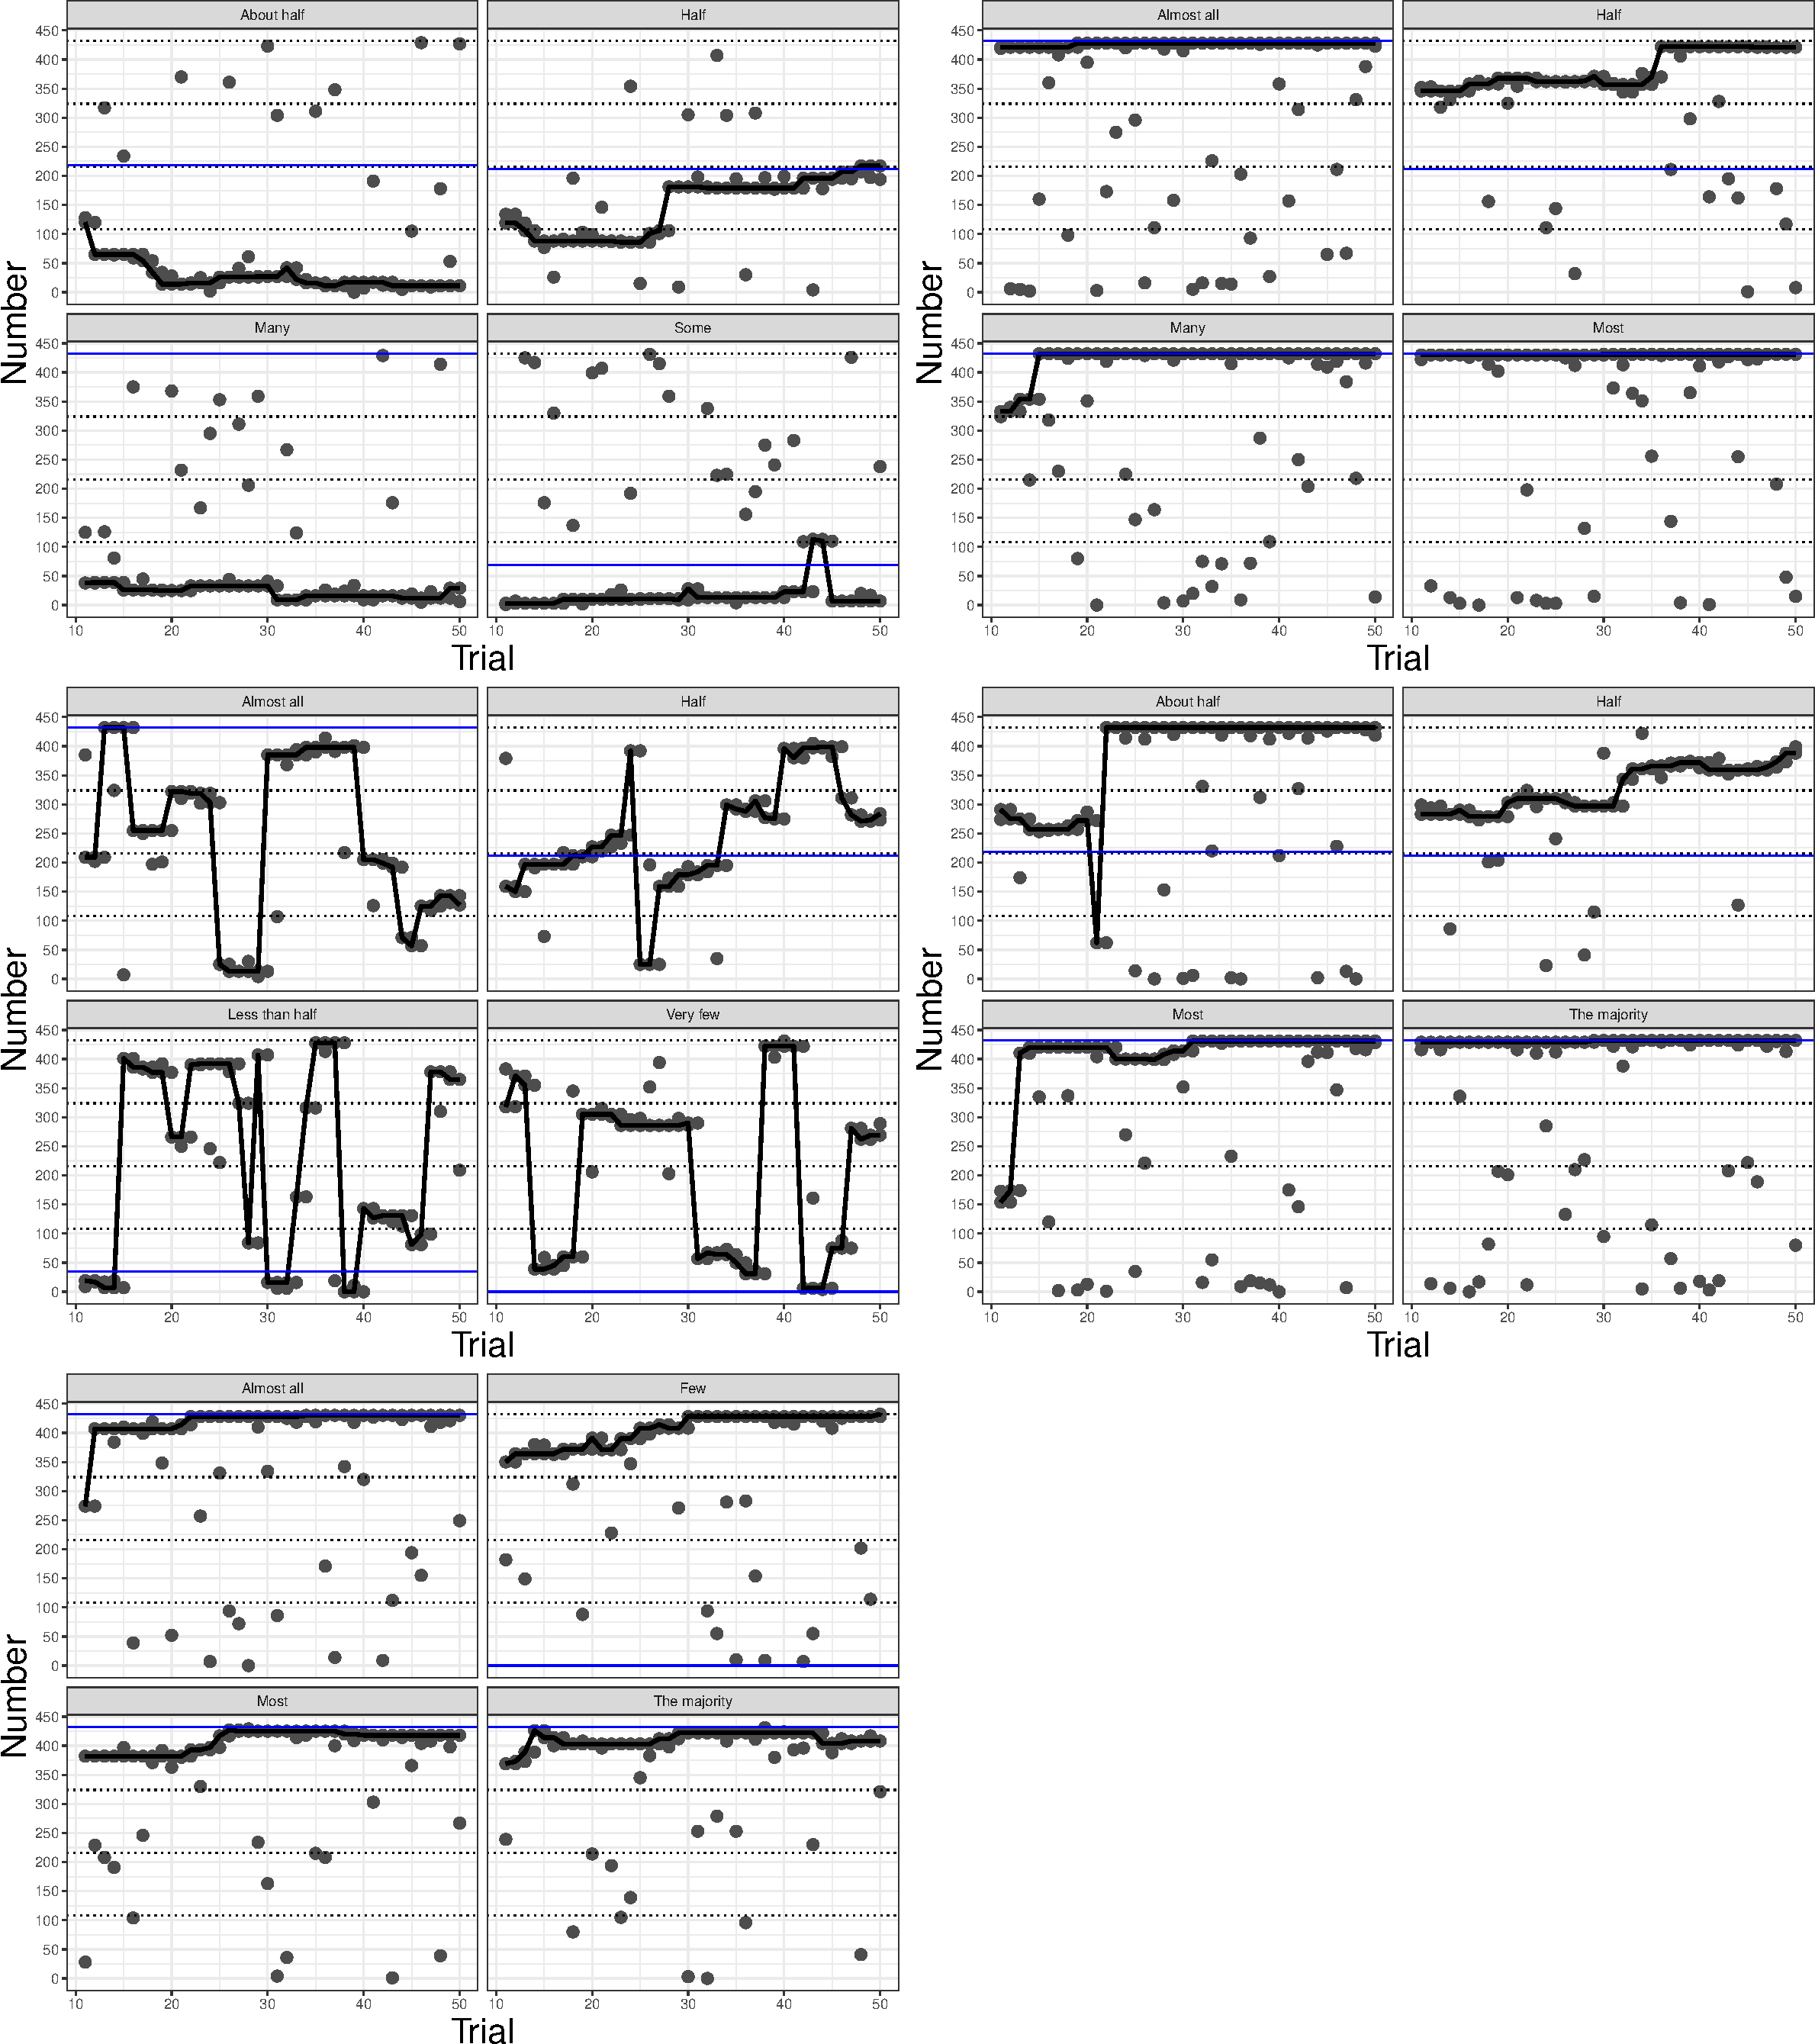
\includegraphics{manuscript_files/figure-latex/unnamed-chunk-12-1.pdf}
  \caption{\label{fig:unnamed-chunk-12}Raw data for the excluded participants.
  Blue line indicates the mode of the subjective probability distribution
  for that specific quantifier (estimated without excluded participants).}
  \end{figure}
  
  \hypertarget{refs}{}
  \end{appendix}

\end{document}
